В данной работе предлагается новый подход к предсинтаксическому аннотированию текста на естественном языке. Данный подход отличается от существующих тем, что: 
\begin{itemize}
\item
позволяет аннотировать текст, содержащий дефекты;
\item
универсален для разных языков;
\item
допускает неоднозначность результата аннотирования.
\end{itemize}
В случае разметки текста по правилам, такие дефекты, как пропущенные или, наоборот, лишние разделительные символы, не могут быть учетны ввиду того, что алгоритмы разметки текста, использующие регулярные выражения, ориентируются на непосредственное присутствие того или иного символа или символа, принадлежащего какому-либо типу. Универсальность разработанного подхода выражается в том, что модуль, разработанный на основе данного подхода может быть адаптирован для работы с несколькими языками без изменения кода самого модуля. Адаптирование заключается в обучении модуля на той или иной тренировочной выборке и в предоставлении необходимых ресурсов: морфологического словаря и частотных списков n-грамм.
Предлагаемый подход состоит из двух фаз:
\begin{itemize}
\item
фаза разметки текста;
\item
фаза словарного поиска.
\end{itemize}
Для предварительной разметки текста введена фаза разметки текста. По-другому задача разметки текста называется графематическим анализом. Предварительная разметка текста представляет собой поиск границ токенов. Другими словами, задача, выпоняемая на фазе разметки текста состоит в преобразовании последовательности символов, представляющей текст на естественном языке, в последовательность найденных токенов. Токенами могут быть словоформы и цифровые комплексы. Следует подчеркнуть, что результат работы фазы разметки текста однозначен, т.е. для данной последовательности символов текста может быть получена одна и только одна последовательность токенов. 
\begin{figure}[H]
	\centering
	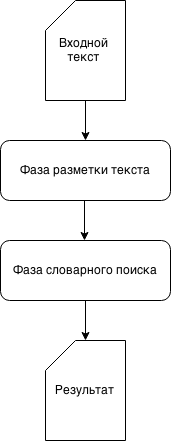
\includegraphics[scale=0.7]{img/approach.png}
	\caption{Фазы разработанного подхода}
\end{figure}
Впоследствии результат, полученный на фазе разметки текста, передается на вход фазе словарного поиска. Фаза словарного поиска введена для достижения учета возможности наличия в тексте дефектов. Для установления корректности найденных словоформ введена фаза словарного поиска. Задача фазы словарного поиска - установить корректность найденных словоформ путем их поиска в словаре и, в случае неудачного поиска, найти возможные варианты корректировки.

\subsection{Фаза разметки текста}
Фаза разметки текста выполняет предварительную разметку текста. Для достижения возможности адаптирования разработанного программного модуля для работы с разными языками на данной фазе принято решение использовать алгоритм, относящийся к классу алгоритмов машинного обучения. Была проанализирована сущность процесса разделения последовательности символов на отдельные единицы - токены. С одной стороны, данный процесс может быть представлен конечным автоматом и описан некоторой формальной грамматикой. Такой взгляд на данный процесс носит детерменированный характер и требует четкого задания формальной грамматики, что может представлять дополнительную трудоемкость при адаптации модуля для работы с текстами на разных языках. С другой стороны, процесс разделения последовательности символов на отдельные единицы может быть рассмотрен как стохастический, причем двойственный. Во-первых, мы имеем непрерывню последовательность символов. А во-вторых, данная последовательность представляет последовательность токенов. Связь этих двух последовательностей можно рассмотреть с вероятностной точки зрения. Данный взгляд на процесс разделения последовательности символов хорошо отображается семантикой скрытой марковской модели. Исходя из этого, было принято решение использовать скрытую марковскую модель (СММ). 

Использование СММ предполагает подбор параметров модели, хорошо правдоподобно описывающих процесс. Подбор параметров представляет собой обучение модели. В данной работе используется алгоритм обучения с учителем. Для работы алгоритма обучения с учителем необходимо прдоставить обучающее множество. Формирование обучающего множества является частью работы и выполняется на основе использования размеченного лингвистического корпуса. Обученная скрытая марковская модель используется для анализа входного текста и выполнения предварительной разметки текста.

\begin{figure}[H]
	\centering
	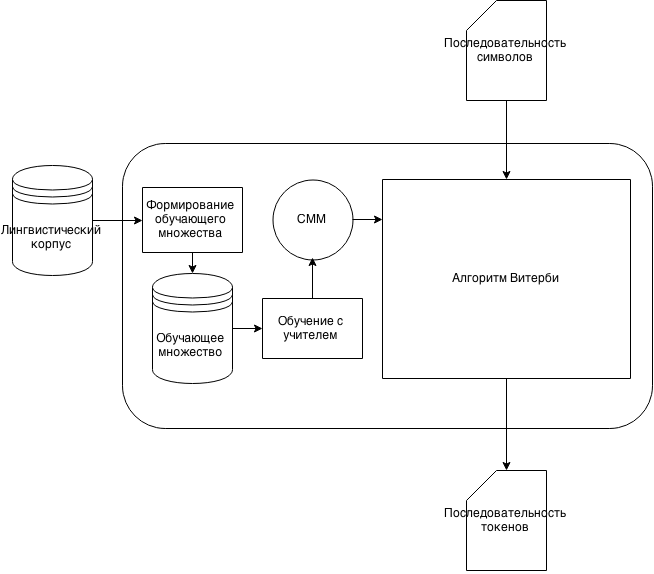
\includegraphics[scale=0.7]{img/tokenization.png}
	\caption{Фаза разметки текста}
\end{figure}

\subsubsection{Скрытая марковская модель}
Скрытая марковская модель - статистическая модель, широко применяемая в задачах распознавания речи, биоинформатики, сжатия данных, а также в области искуственного ителлекта. Процессы, протекающие в реальном мире проявляются в виде сигналов, воспринимаемых наблюдателем. Нередко источник сигналов непостижим наблюдателем в явном виде. Наблюдатель может судить о состоянии источника сигнала лишь по полученным сигналам, которые могут быть подвержены влиянию шумов, вследствие чего задача определения состояния источника сигналов становится нетривиальной. СММ является вероятностной моделью, широко применяемой в задачах определения внутреннего состояния процессу по его внешним проявлениям. СММ представляет собой обучаемый стохастический конечный автомат и может быть рассмотрены как специфическая форма динамической байесовской сети.

Впервые скрытые марковские модели начали применяться в области распознавания речи. Историю СММ можно разделить на две части. \cite{kouemou} С одной стороны это история Марковского процесса и Марковских цепей, а с другой - история алгоритмов, разрабатывавшихся для решений различных задач с помощью СММ. Андрей Андреевич Марков описал Марковские цепи в 1906 г., когда получил первые теоретические результаты исследования стохастических процессов. Марковский процесс может быть рассмотрен как процесс изменения некоторой случайной величины, который удовлетворяет Марковскому свойству. Марковское свойство заключается в том, что условное распределение вероятностей будущих состояний зависит от состояния, в котором процесс находится на данный момент, и не зависит от предыстории состояний. Другими словами, будущее не зависит от прошлого и зависит только от настоящего. В 1940-е годы с бурным развитием компьютерных наук многие ученые из разных областей начали искать применение как детерменированных, так и стохастических автоматов для решения своих задач. В 1977 году были обобщены накопившиеся знания и опыт использования EM-алгоритма \cite{dempster1977maximum}. 

EM-алгоритм является классическим алгоритмом, используемым в математической статистике для нахождения максимально правдоподобной оценки неизвестных параметров вероятностных моделей. EM-алгоритм представляет собой итеративный алгоритм.Каждая итерация алгоритма состоит из двух шагов. На E-шаге (expectation) вычисляется ожидаемое значение функции правдоподобия, при этом скрытые переменные рассматриваются как наблюдаемые. На M-шаге (maximization) вычисляется оценка максимального правдоподобия, таким образом увеличивается ожидаемое правдоподобие, вычисляемое на E-шаге. Затем это значение используется для E-шага на следующей итерации. Алгоритм выполняется до сходимости. Алгоритм Баума-Велша является частным случаем EM-алгоритма и применяется для нахождения неизвестных параметров скрытой марковской модели. Алгоритм Витерби был предложен Эндрю Витерби в 1967 году для декодирования сверточных кодов \cite{viterbi1967error}. Этот алгоритм относится к классу алгоритмов динамического программирования и позволяет найти наиболее правдоподобную последовательность скрытых состояний процесса, называемую путем Витерби.

\paragraph{Математическая модель}
Скрытая марковская модель представляет собой обучаемый стохастический конечный автомат. Выделяют два вида СММ: для дискретных наблюдений(событий) и непрерывных сигналов. В работе рассмотрена дискретная СММ ввиду дискретного характера данных, что будет обосновано далее. Скрытая марковская модель объединяет в себе два стохастических процесса.
\begin{itemize}
\item
Первый процесс представляет собой переходы между состояними, скрытыми от наблюдателя.
\item
Второй процесс представляет собой пояление некоторый событий, которые известны наблюдателю. Распределения вероятностей появления этих событий зависят от скрытого состояния, в котором находится система.
\end{itemize}


Формальо модель может быть описана следующими математическими объектами:
\begin{itemize}
	\item
	Количество скрытых состояний модели \(N\). Несмотря на то, что информация о том, в каком состоянии модель находится в конкретный момент времени, не доступна для наблюдателя, множество всевозможных состояний наблюдателю извествно:
	множеством скрытых состояний
	\[ S = \{ S_1, S_2, ..., S_N \};\]
	\item
	Количество различных символов наблюдений \(M\). Символы наблюдений соответствуют регистрируемым событиям, попрождаемым наблюдаемым процессом. Множество различных символов наблюдений называется алфавитом наблюдений
	\[ V = \{ v_1, v_2, ..., v_M \};\]
	\item
	Матрицей вероятностей переходов между скрытыми состояниями
	\begin{align} 
		&A = \{ a_{ij} \}, \nonumber \\
		&a_{ij} = P[q_{t + 1} = S_j | q_t = S_i]; \nonumber
	\end{align}
	\item
	Распределение вероятностей появления символов в j-ом состоянии
	\begin{align}
		&B = \{ b_j(k) \}; \nonumber \\ 
		&b_j(k) = P(v_k | t = k, q_t = S_j); \nonumber
	\end{align}
	\item
	Распределение вероятностей начального состояния
	\begin{align}
		&\pi = \{\pi_i\}; \nonumber \\
		&\pi_i = P(q_1 = S_i). \nonumber
	\end{align}
\end{itemize}

Таким образом, чтобы полностью задать СММ необходимо определить параметры модели (\(N, M\)), определить алфавит символов наблюдений и вероятностные характеристики модели \(A, B\) и \(\pi\). Для компактной записи полного задания параметров модели используется нотация
\[\lambda = (A, B, \pi).\]

Определены три типовые задачи, решаемые при импользовании СММ в различных прикладных задачах \cite{Rabiner89atutorial}:
\begin{itemize}
	\item
	Вычисление \(P(O|\lambda)\), вероятности проявления поледовательности событий, при данных последовательности событий \(O=O_1O_2...O_T\) и модели \(\lambda = (A, B, \pi)\);
	\item
	Выбор последовательности скрытых состояний \(Q=q_1q_2...q_T\), которая наилучшим образом объяняет последовательность наблюдений, при данных последовательности событий \(O=O_1O_2...O_T\) и модели \(\lambda = (A, B, \pi)\);
	\item
	Подбор параметров модели \(\lambda = (A, B, \pi)\) для максимизации \(P(O|\lambda)\).
\end{itemize} 

Другими словами первую задачу можно определить как определение вероятности того, что полученная последовательность наблюдений порождена данной моделью. С другой стороны, решение данной задачи может потребоваться для оценки правдоподобия подобранных параметров модели, что может потребоваться при решении задачи подбора параметров модели или выбора конкретной модели из нескольких. Первая задача решается с помощью алгоритма ``прямого-обратного'' хода. Данный алгоритм имеет вычислительную сложность \(O(T * N^T)\), где \(T\) - длина последовательности, \(N\) - число скрытых состояний модели. Решение второй задачи представляет собой постижение скрытого процесса. Другими словами решение данной задачи позволяет найти наиболее вероятную последовательность скрытых состояний системы по имеющейся последовательности наблюдений. Последовательность скрытых состояний модели называется путем Витерби, для нахождения которого используется алгоритм Витерби, имеющий вычислительную сложность \(O(T * |S|^2)\), где \(|S| = N\) - количество скрытых состояний модели, а \(T\) - размер входной последовательности наблюдений. Здесь следует отметить, что в применении к конкретной задаче количество скрытых состояний может быть определено, т.е. быть величиной постоянной, а значит согласно правилам асимптотической оценки \cite{clrs} сложности алгоритмов, сложность алгоритма Витерби линейна относительно размера входной последовательности. Третья задача является задачей оптимизации параметров модели с целью наилучшего объяснения наблюдаемых последовательностей событий. По-другому данная задача называется задачей обучения, причем данный вид обучения является обучением без учителя и решается с помощью алгоритма Баума-Велша.

Приведем пример системы, описываемой скрытой марковской моделью. Пусть в комнате находятся два человека. У первого человека завязаны глаза, перед вторым человеком стоят \(N\) урн, наполненных шарами разного цвета. Второй человек начинает брать шары из разных урн в произвольном порядке и называть цевета взятых шаров. При этом он не говорит из какой именно урны он взял тот или иной шар. 
\begin{figure}[H]
	\centering
	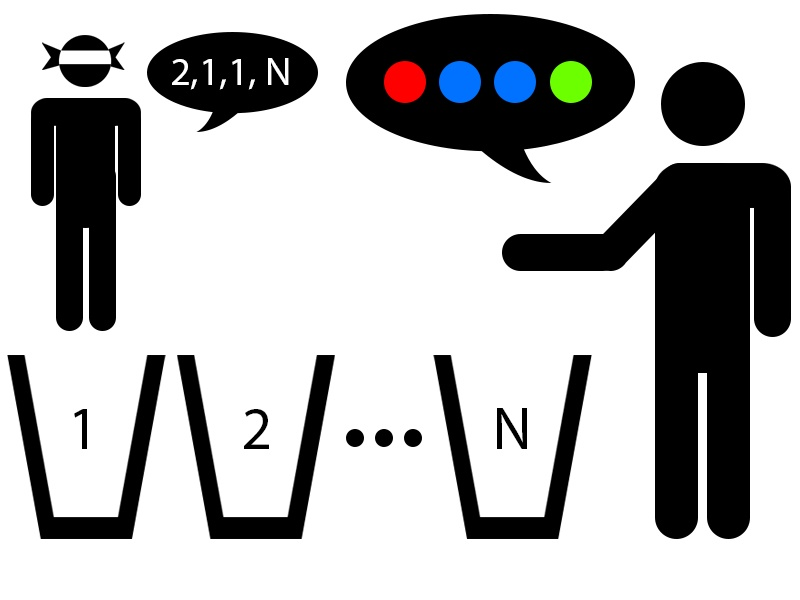
\includegraphics[scale=0.7]{img/hmm.jpg}
	\caption{Иллюстрация процесса, описываемого СММ}
\end{figure}
Используя СММ для описания этого процесса первый человек может пытаться угадывать, из какой урны, какой шар был взят. Наблюдаемым процессом в данном случае является речь человека, называющего цвета взятых шаров, а скрытым процессом являетсе его выбор той или иной урны. В этой ситуации элементами множества наблюдений являются цвета шаров, а элементами множества скрытых состояний являются номера урн.

\subsubsection{Использование скрытой марковской модели для разметки текста}
Текст на естественном языке так же можно рассматривать как два стохастических процесса, описываемых скрытой марковской моделью. В таком случае наблюдаемым процессом можно считать последовательность символов текста, а скрытым процессом - принадлежность того или иного символа словоформе, ее границе или непринадлежность символа словоформе. Возможно введение дополнительных скрытых состояний для описания различных типов словоформ. Множество наблюдений представляет собой типы символов, из которых состоит текст. В простейшем случае множество наблюдений может представлять собой подмножество кодов символов некоторого набра символов, например, Юникода.
\begin{itemize}
	\item
	Определим множество скрытых состояний:
	\begin{align*}
		&S = \{ S_{in}, S_{out}, S_{bnd}\}, \text{где}\\
		&S_{in} - \parbox[t]{20em}{состояние, соответсвующее расположению символа внутри словоформы,} \\
		&S_{out} - \parbox[t]{20em}{состояние, соответсвующее расположению символа вне словоформы,} \\
		&S_{bnd} - \parbox[t]{20em}{состояние, соответсвующее расположению символа на границе словоформы.} \\
	\end{align*}

	\item
	Определим множество наблюдений:
	\begin{align*}
		&V = \{ v | v \in C\}, \text{где} \\
		&C - \parbox[t]{25em}{некоторое подмножество символов Юникода}
	\end{align*}
\end{itemize}

Для полного определения скрытой марковской модели, которую можно использовать для разметки текста, необходимо также задать матрицу вероятностей переходов между скрытыми состояниями \(A\), вектор распределений вероятностей появления символов \(B\) и распеределение вероятностей начального состояния \(\pi\). Для подбора данных параметров модели необходимо прменение какого-либо метода обучения. В работе применяется метод обучения с учителем, который рассомтрен в следующем разделе.

\subsubsection{Обучение скрытой марковской модели с учителем}
Как было упомянуто выше, алгоритм Баума-Велша является обучением без учителя. В данном алгоритме производится подбор параметров модели для достижения наиболее правдоподобного соответствия последовательности скрытых состояний \(Q=q_1q_2...q_T\) последовательности наблюдений \(O=O_1O_2...O_T\). При отстутсвии каких-либо начальных сведений о вероятностях переходов между состояниями или распределениях вероятнстей появлений символов для различных скрытых состояний, данный алгоритм позволит обучить модель для распознавания моментов смены скрытых состояний, однако сами состояния не будут привязаны к конкретному типу.

В данной работе используется метод обучения скрытой марковской модели с учителем. Метод основан на частотном определении вероятности. Для обучения используется обучающая выборка или обучающее множество, представляющее собой множество множество пар последовательностей наблюдений и соответствующих им последовательностей скрытых состояний. Принимая на вход обучающую выборку, алгоритм обучения производит подбор параметров модели. Опишем работу алгоритма. Пусть дано обучающее множество
\begin{align*}
T = \{(O_i, Q_i) | 0 \le i \le N\} \text{,}
\end{align*}
где \(N\) - количество элементов обучающего множества. Для \(z\) от \(0\) до \(N\) необходимо
\begin{itemize}
\item
инкрементировать \(\pi_i\), где \(O_{z0}\) = \(S_i\);
\item
прибавить к \(a_{ij}\) число, равное количеству переходов из состояния \(S_i\) в \(S_j\) в данной последовательности;
\item
прибавить к \(b_j(k)\) количество появлений символа \(V_k\) в состоянии \(S_j\).
\end{itemize}
Так как может оказаться, что некоторые элементы \(\pi_i = 0\), \(a_{ij} = 0\) или \(b_j(k) = 0\), то необходимо произвести корректировку, которая заключается в прибавлении \(1\) ко всем элементам.
Теперь можно вычислить окончательные параметры модели следующим образом:
\begin{itemize}
\item
\(\pi_i \leftarrow \frac{\pi_i}{\displaystyle\sum_{k} \pi_k} \);
\item
\(a_{ij} \leftarrow \frac{a_{ij}}{\displaystyle\sum_{k} a_{ik}} \);
\item
\(b_j(k) \leftarrow \frac{b_j(k)}{\displaystyle\sum_{t} b_j(t)} \).
\end{itemize}

\subsubsection{Формирования обучающего множества}
В предыдущем разделе был рассмотрен алгоритм обучения скрытой марковской модели с учителем, который применяется в данной работе. Данный алгоритм принимает на вход тренировочное множество, на основе которого выполняется обучение модели. Исходя из этого, необходимо решить задачу о составлении тренировочного множества.


\subsection{Фаза словарного поиска}
Фаза словарного поиска принимает на вход результат разметки текста, полученный на фазе разметки текста. Как было сказанно выше, результатом работы первой фазы является список найденных токенов. Задача фазы словарного поиска проверить корректность найденных токенов и, возможно, произвести коррекцию результата. Рузультат может быть неоднозначным. Т.е. возможно существование нескольких вариантов разбиения исходной последовательности символов на токены. 

Для реализации 

\subsubsection{Графовый словарь}
Разработанный в данной работе подход применяется в программном модуле, входящем в состав системы семантического анализа. Данная система семантического анализа основана на такой лингвистической концепции, как фреймовая семантика \cite{fillmore1976frame}. Используемые алгоритмы анализа текста работают с внутренним словарем, имеющим графовую структуру. Данный словарь объединяет в себе морфологический словарь и семантическую сеть. В рамках графовой структуры словаря определены узлы трех типов:
\begin{itemize}
	\item
	семантические узлы;
	\item
	узлы лексем;
	\item
	узлы словоформ.
\end{itemize}
Узлы графового словаря связаны ребрами следующих типов:
\begin{itemize}
	\item
	ребра, соответствующие семантическим отношениям;
	\item
	ребра, связывающие семантические узлы с узлами лексем и выражающие возможность представления того или иного понятия конкретной лексемой в тексте;
	\item
	ребра, связвающие лексемы с их словоформами.
\end{itemize}
Семантический узел представляет собой синонимический ряд (``синсет'' \cite{wordnet}). Семантические узлы могут быть связаны ребрами, выражающими такие семантические отношения, как:
\begin{itemize}
\item
гиперонимия;
\item
гипонимия;
\item
``часть -- целое'';
\item
меронимия;
\item
антонимия;
\item
и др.
\end{itemize}
Результатом работы модуля аннотирования является список найденных токенов, представляющий собой ссылки на найденные словоформы.
\begin{figure}[H]
	\centering
	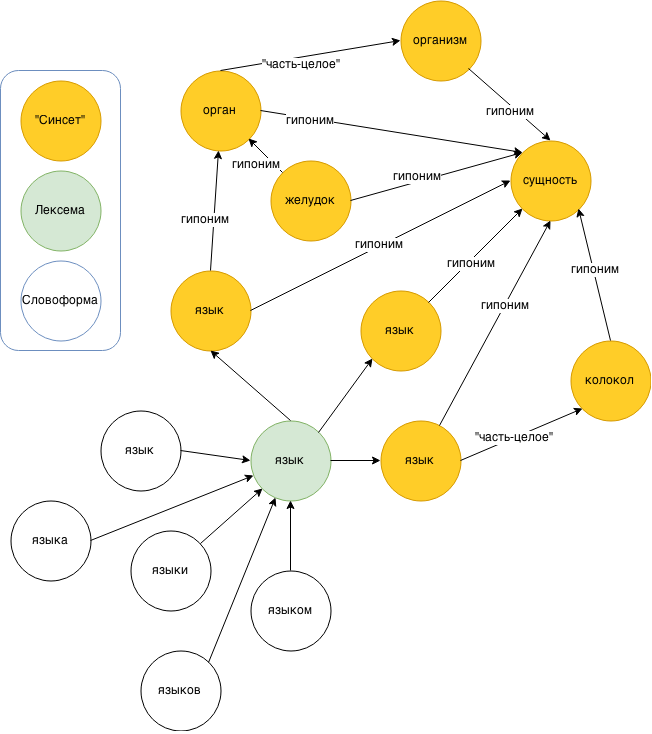
\includegraphics[scale=0.5]{img/dict.png}
	\caption{Пример фрагмента графового словаря}
\end{figure}

\subsubsection{Дерево поиска}
Алгоритмы, используемые на данной фазе работают с графовым словарем. Для избежания полного сканирования узлов словоформ во время операций прямого и нечеткого поиска по словарю, используется префиксное дерево поиска.

\subsubsection{Расстояние Левенштейна}
\subsubsection{Алгоритм поиска}
\subsubsection{Ранжирование результатов}